\chapter[Introduction]{Introduction}
\label{chap:intro}


%intorduccion del trabajo a realizar
%motivacion
%introducir proyecto en el que trabajas
%intruducir la empresa




\section{Context: Importance of Air Quality (Health, Climate, Policy)}
Air pollution has become one of the major environmental challenges of the 21st century. Poor air quality has direct impacts on human health, contributing to respiratory and cardiovascular diseases, and is linked to millions of premature deaths globally each year. Furthermore, atmospheric pollutants such as ozone (O$_3$), nitrogen dioxide (NO$_2$), and particulate matter (PM$_{2.5}$, PM$_{10}$) affect ecosystems, agriculture, and play a role in climate change processes. For this reason, monitoring and forecasting air quality has become an essential tool in environmental policy, public health planning, and citizen awareness.  

The urgency of this challenge is also recognized at the political and institutional level. Within the framework of the United Nations 2030 Agenda for Sustainable Development, several goals are directly related to the problem of air pollution. Goal 3 (Good Health and Well-Being) emphasizes the need to reduce illnesses caused by hazardous chemicals and air pollution; Goal 11 (Sustainable Cities and Communities) calls for improving urban air quality and reducing environmental impacts of cities; and Goal 13 (Climate Action) highlights the interconnections between air pollutants, greenhouse gases, and the fight against climate change. The European Union has also aligned its environmental policies with these objectives, reinforcing the importance of reliable air quality data for informed decision-making.


Here we have an image to the referenced goals \ref{fig:ej1}. A link to \href{https://sdgs.un.org/goals}{Sustainable development goals}%\footnotemark. 


\begin{figure} [h!btp]
	\centering
	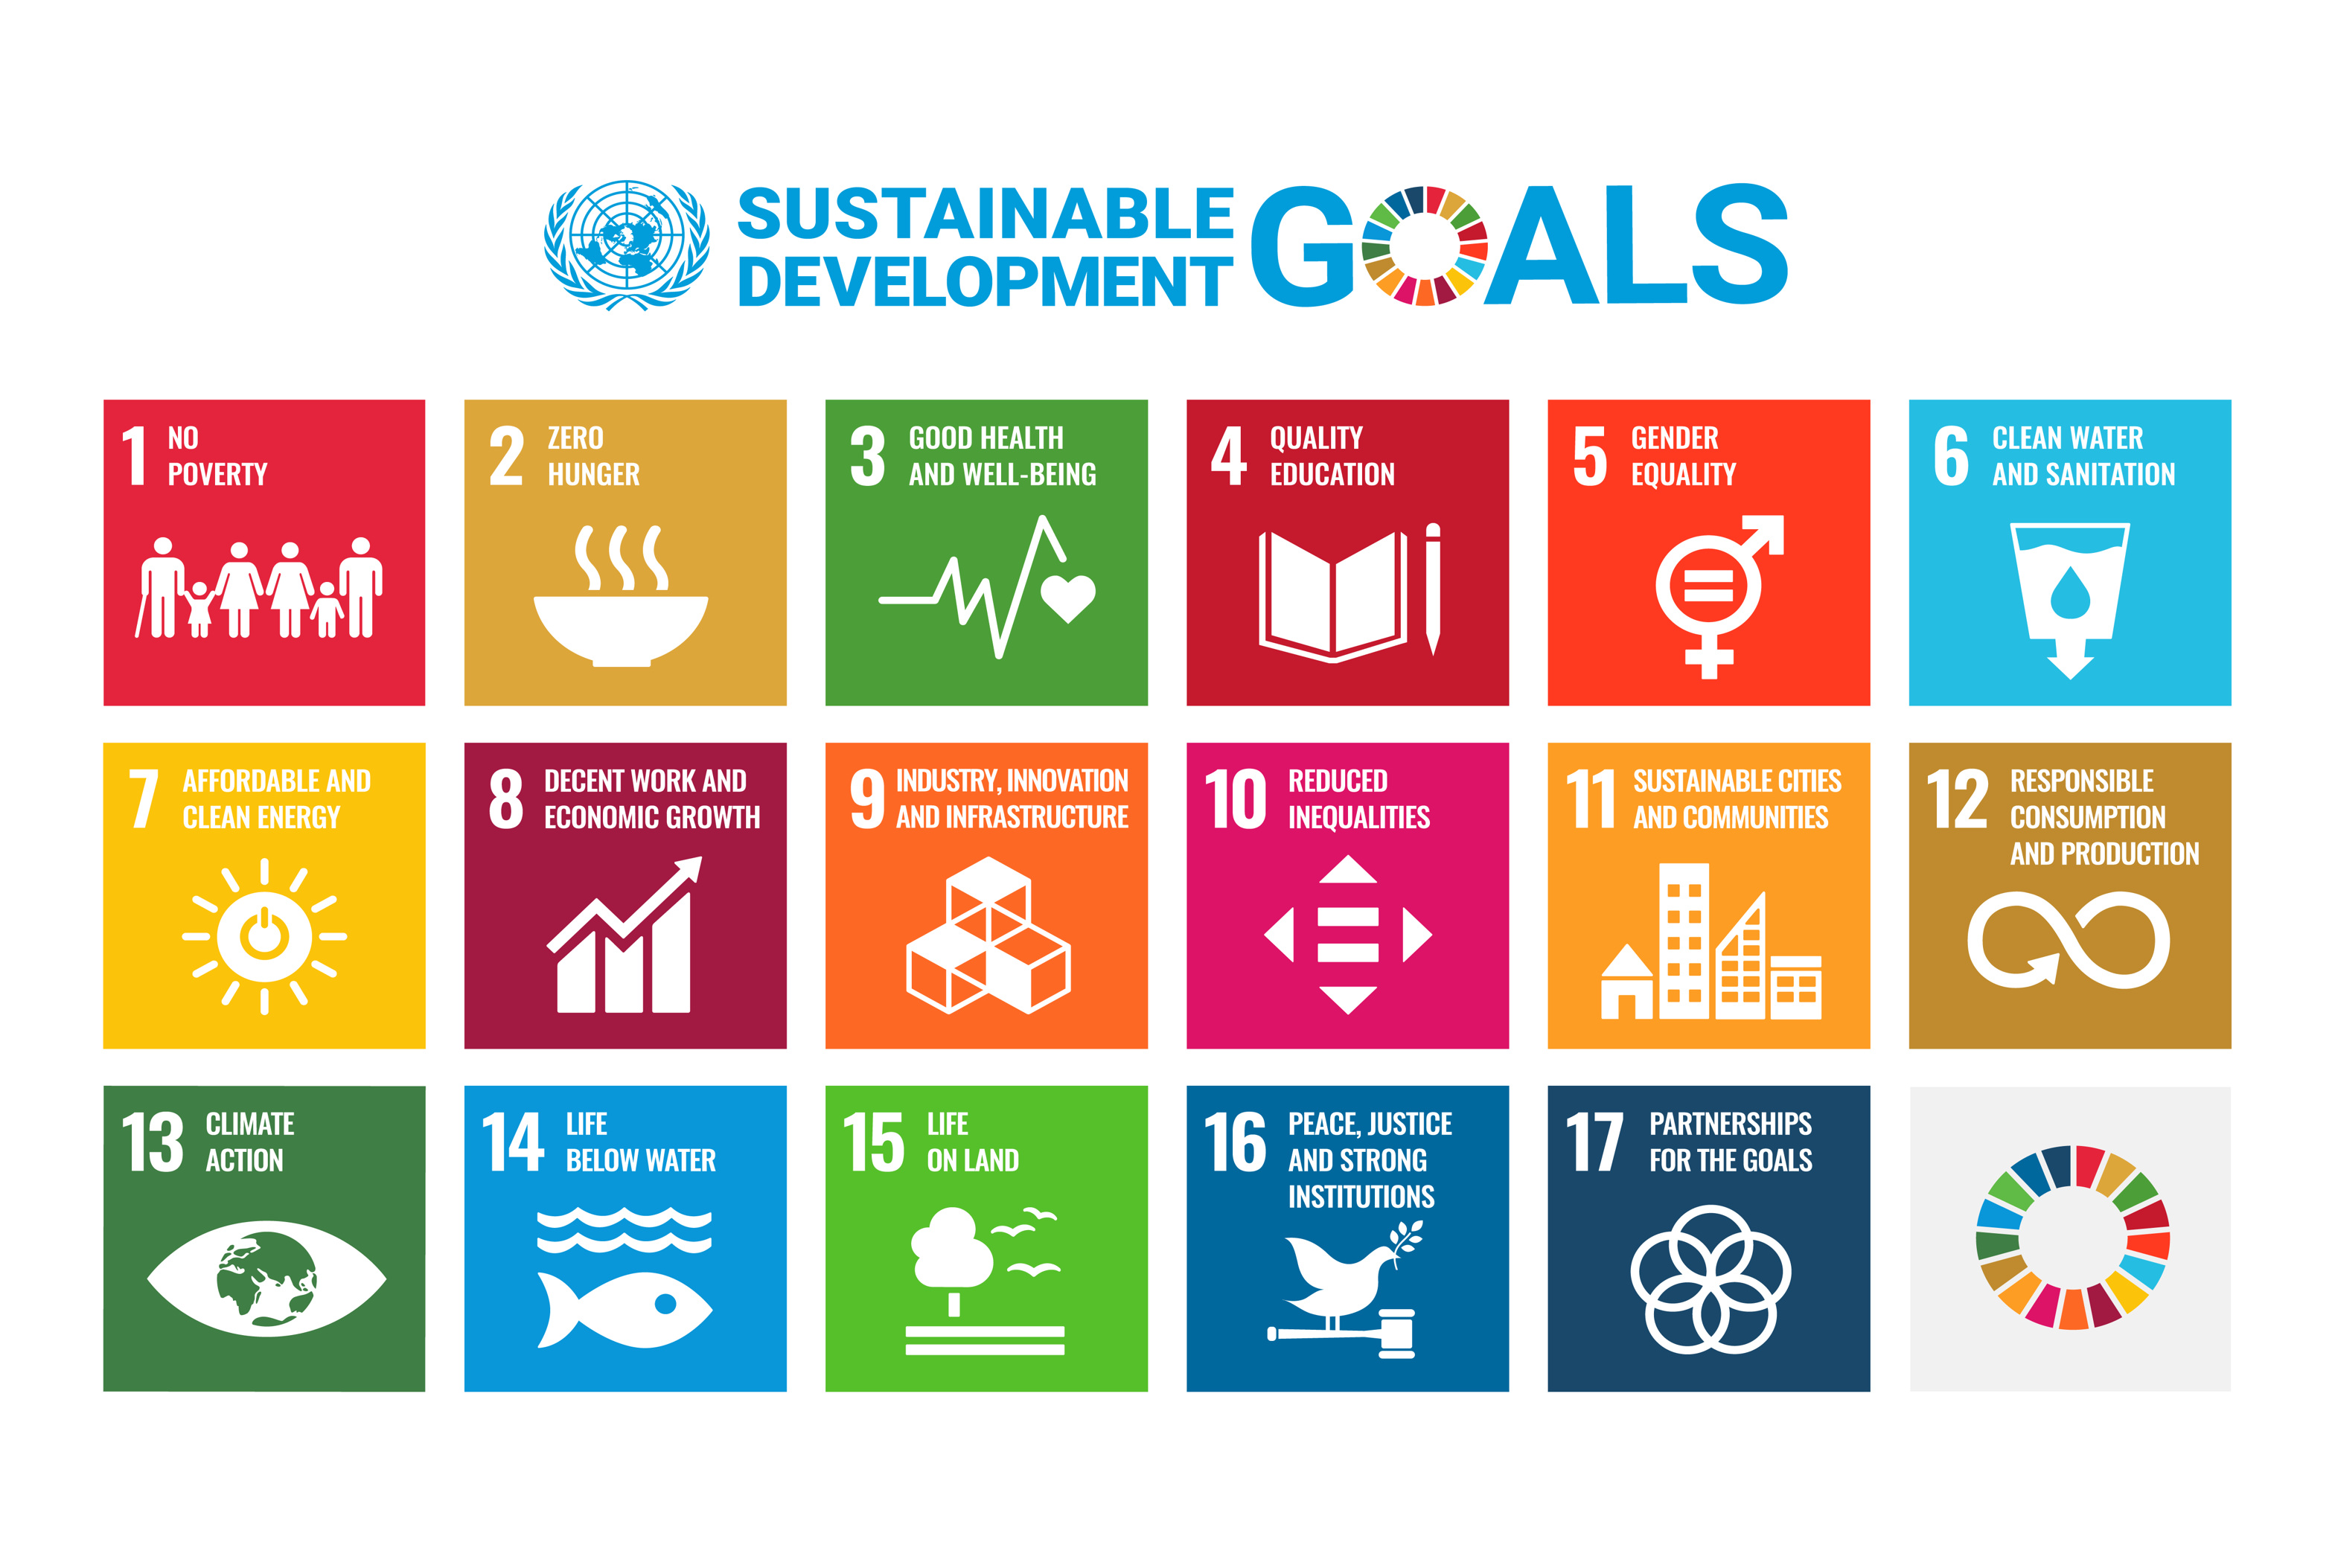
\includegraphics[width=0.7\textwidth]{fig/sustainable-image.png}
	\caption[Sustainable development goals]{Sustainable development goals\footnotemark}
	\label{fig:ej1}
\end{figure}
\footnotetext{https://sdgs.un.org/goals}

\section{The Role of CAMS in Air Quality Forecasting}

The Copernicus Atmosphere Monitoring Service (CAMS), operated by the European Centre for Medium-Range Weather Forecasts (ECMWF), provides high-resolution global and European air quality forecasts based on advanced atmospheric models and satellite data. CAMS combines chemical transport models, meteorological predictions, and data assimilation techniques to deliver near real-time and forecasted atmospheric composition data, including concentrations of pollutants such as PM$_{2.5}$, O$_3$, NO$_2$, and more. This makes CAMS a key infrastructure for researchers, decision makers, and developers working on climate and environmental services.

Here we have CAMS logo \ref{fig:ej2}. A link to  \href{https://atmosphere.copernicus.eu/}{CAMS webpage}%\footnotemark. 


\begin{figure} [h!btp]
	\centering
	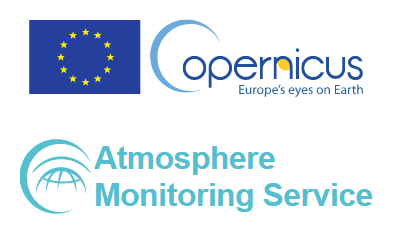
\includegraphics[width=0.7\textwidth]{fig/copernicus-image.png}
	\caption[CAMS]{CAMS\footnotemark}
	\label{fig:ej2}
\end{figure}
\footnotetext{https://atmosphere.copernicus.eu/}

\section{Motivation: Combining Visualization and Technical Analysis}

However, while CAMS offers a wide range of high-quality data products, their accessibility for non-experts is limited. Existing tools are often either too technical, sometimes providing raw WMS layers with little interactivity or only too simplified, focusing only on summary indicators like the Air Quality Index (AQI). This project is motivated by the desire to bridge this gap through the development of a visualization tool that can display CAMS forecast data in an intuitive, interactive way. 

\section{Objectives of the Project}

At the same time, the project aims to analyze how CAMS models generate their predictions and how their performance is evaluated using real-world observations.
The main objectives of this project are therefore:

\begin{itemize}
	\item To understand how CAMS forecasting models operate, including their input data, algorithms, and structure.
	\item To explore the evaluation methods used to assess the accuracy and reliability of air quality forecasts.
	\item To develop a web-based visualization tool that displays CAMS air quality forecast data in a user-friendly, informative manner.
\end{itemize}
